%!TEX program = pdflatex

\documentclass[a4paper, 12pt]{article}

\usepackage{geometry}
\geometry{a4paper,
total={170mm,257mm},left=2cm,right=2cm,
top=1cm,bottom=2cm}

\usepackage{mathtext}
\usepackage{amsmath}
\usepackage[T2A]{fontenc}
\usepackage[utf8]{inputenc}
\usepackage[english,russian]{babel}
\usepackage{graphicx, float}
\usepackage{tabularx, colortbl}
\usepackage{caption}
\captionsetup{labelsep=period}

\newcommand{\parag}[1]{\paragraph*{#1:}}
\DeclareSymbolFont{T2Aletters}{T2A}{cmr}{m}{it}
\newcounter{Points}
\setcounter{Points}{1}
\newcommand{\point}{\arabic{Points}. \addtocounter{Points}{1}}
\newcolumntype{C}{>{\centering\arraybackslash}X}

\begin{document}
%\maketitle

\begin{titlepage}
    \vspace*{\fill}
    
    \begin{center}
        
\includegraphics[scale=0.8]{res/MIPT.pdf}
        \\[0.7cm]\Huge Московский Физико-Технический Институт
        \\[2cm]\LARGE Отчет о выполнении лабораторной работы 
        \\[0.5cm]\noindent\rule{\textwidth}{1pt}
        \\\Huge\textbf{5.10.1 \\ Электронный парамагнитный резонанс}
        \\[-0.5cm]\noindent\rule{\textwidth}{1pt}
    \end{center}
    
    \vspace*{\fill}
    
    \begin{flushleft}
        Выполнили: \hspace{\fill} Группа:
        \\Костылев Владислав\hspace{\fill} Б01-206
    \end{flushleft}
\end{titlepage}

\setcounter{page}{2}


\begin{abstract}
    \textbf{Цель работы:} Исследуется электронный парамагнитный резонанс в молекуле ДФПГ, определяется $g$-фактор электрона, измеряется ширина ЭПР. 
\end{abstract}

\tableofcontents
\newpage

\section{Теоретическая справка} 

Энергетический уровень электрона в присутствии магнитного поля с индукцией $B$ расщепляется на подуровня, расстояние между которыми равно 
	\begin{equation}
		\label{eq:dE}
		\Delta E = E_2 - E_1 = 2\mu B.
	\end{equation}
	Здесь $\mu$ -- абсолютная величина проекции магнитного момента на направление поля.
	
	Между этими двумя уровнями возможны переходы. Эти переходы могут возбуждаться внешним высокочастотным электромагнитным полем, если оно имеет нужную частоту и нужное направление.
	
	Резонансное значение частоты определяется из очевидной формулы:
	\begin{equation}
		\label{eq:resonans_omega}
		\hbar \omega_0 = \Delta E.
	\end{equation}

	При переходе с нижнего на верхний уровень энергии электрон поглощает квант электромагнитной энергии, а при обратном переходе такой же квант излучается. Возбуждение электронных резонансных переходов электромагнитным полем, имеющим частоту, определяемую формулой~(\ref{eq:resonans_omega}), носит название электронного парамагнитного резонанса (ЭПР).
	
	В настоящей работе необходимо получить сигнал ЭПР на кристаллическом дифенилпикрилгидразиле (ДФПГ) и определить значение $g$-фактора для электрона. Как известно, связь между магнитным моментом $\mu$ электрона и его механическим моментом $\mathbf{M}$ выражается через гиромагнитное отношение $\gamma$ с помощью формулы
	\begin{equation}
		\label{eq:gyromagnit}
	    \mu = \gamma M.
	\end{equation}
	
	А магнитный момент частицы, измеренный в магнитонах Бора, а механический - в $\hbar$, то их связь можно записать через $g$-фактор:
	\begin{equation}
	    \label{eq:def_g}
	    \frac{\mu}{\mu_\text{Б}} = \frac{M}{\hbar} 
	\end{equation}

	Используя соотношения (\ref{eq:dE})-(\ref{eq:def_g}), нетрудно получить выражение для $g$-фактора через определяемые экспериментально величины:
	\begin{equation}
		\label{eq:g_is}
		\tag{$\star$}
		g = \frac{\hbar \omega_0}{\mu_\text{Б} B}.
	\end{equation}

\newpage


\section {Экспериментальная установка}

    Образец (порошок ДФПГ) в стеклянной ампуле помещяется внутрь катушкииндуктивнсоти входящей в состав колебательного контура. Входящий в состав контура конденсатор состоит из двух платсин, разделенных воздушным зазором, одна из пластин может перемещаться поворотом штока. Колебания в контуре возбуждаются антенной, соединённой с генератором частоты (ВЧ) Г4-116. Амплитуда колебаний поля в катушке индуктивности измеряется по наводимой в петле связи ЭДС индукции. Высокочастотные колебания ЭДС индукции в приёмном контуре детектируются диодом, измеряемая при помощи осциллографа низкочастотная огибающая этого сигнала пропорциональна квадрату амплитуды колебаний поля в катушке.
    \begin{figure}[H]
        \centering
        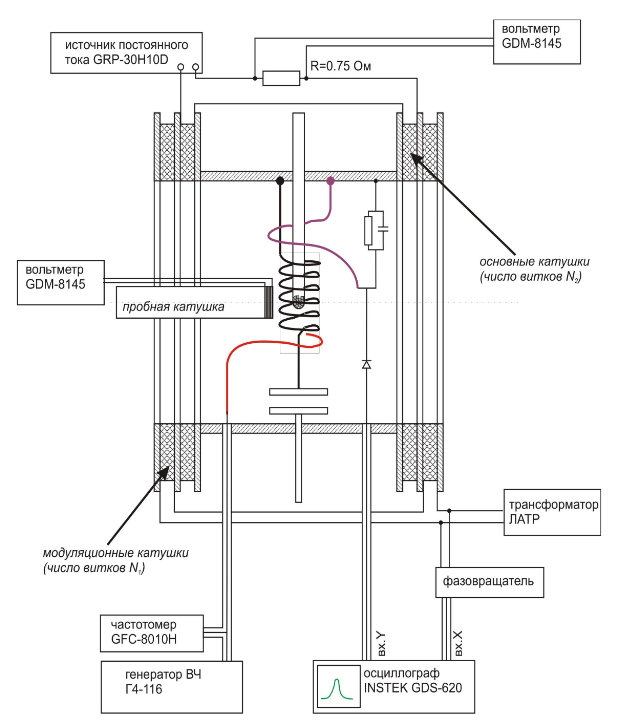
\includegraphics[width=0.7\linewidth]{res/1.png}
    \end{figure}
	
	Постоянной магнитное поле создаётся пропусканием тока от источника постоянного тока через основные катушки. При этом при помощи вольтметра измеряется падение напряжения на резисторе в цепи основных катушек. Переменное поле небольшой амплитуды создаётся подачей на модуляционные катушки напряжения с регулируемого трансформатора ЛАТР. Для измерения амплитуды колебаний переменного поля используется пробная катушка известной геометрии, подключенная к вольтметру.
	
\newpage

    
\section{Результаты измерений и обработка данных} 
    В данной работе мы измерили следующие величины, но сперва мы добились резонанса:
    \begin{figure}[H]
        \centering
        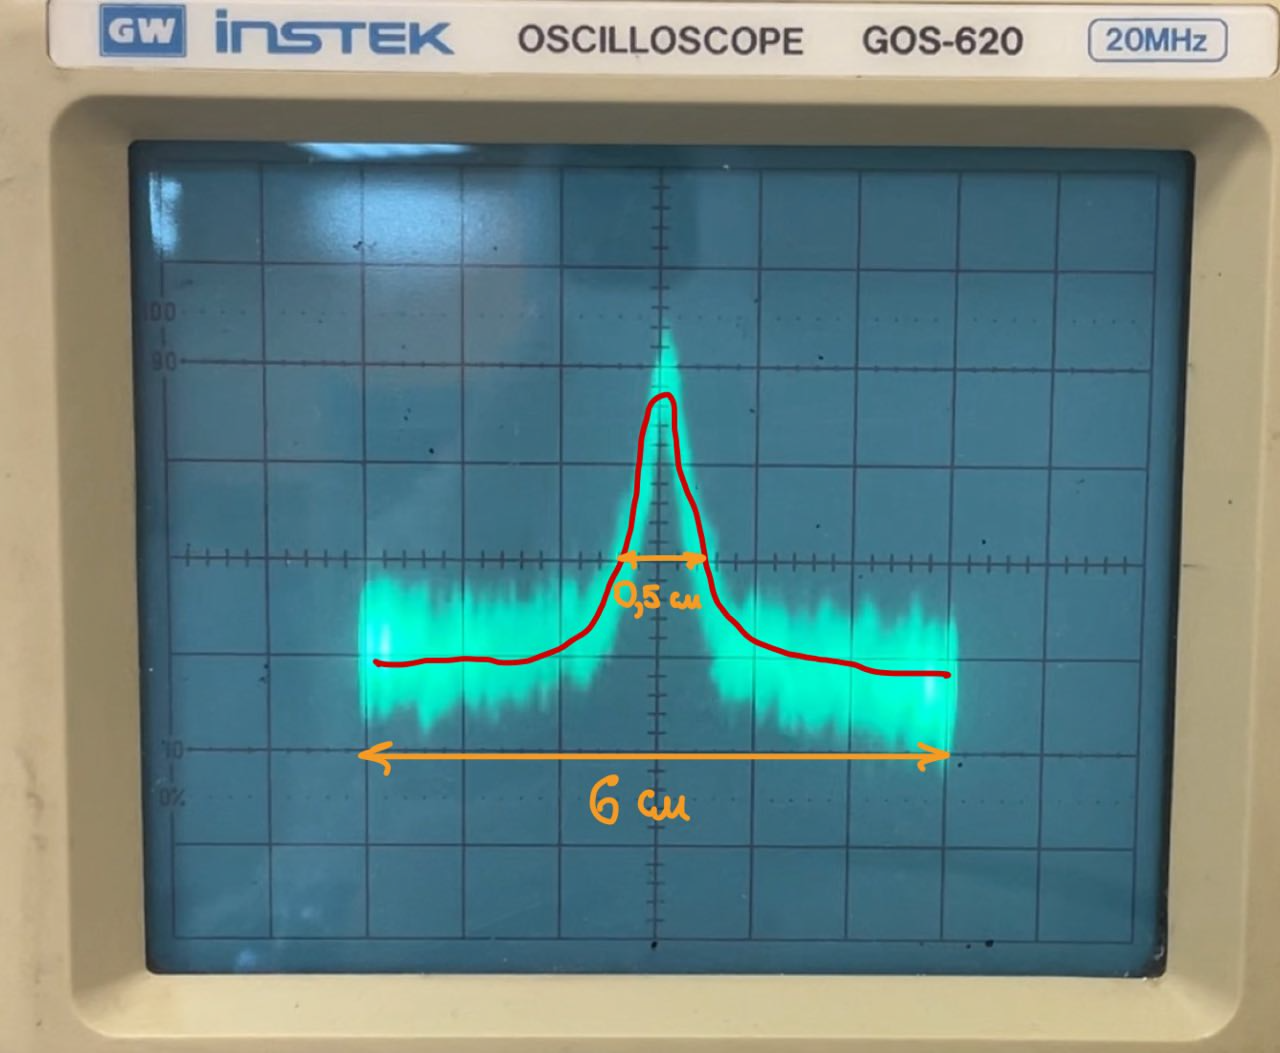
\includegraphics[width=0.6\linewidth]{res/2.png}
    \end{figure}

    Мы рассчитали:
    \begin{figure}[H]
        \centering
        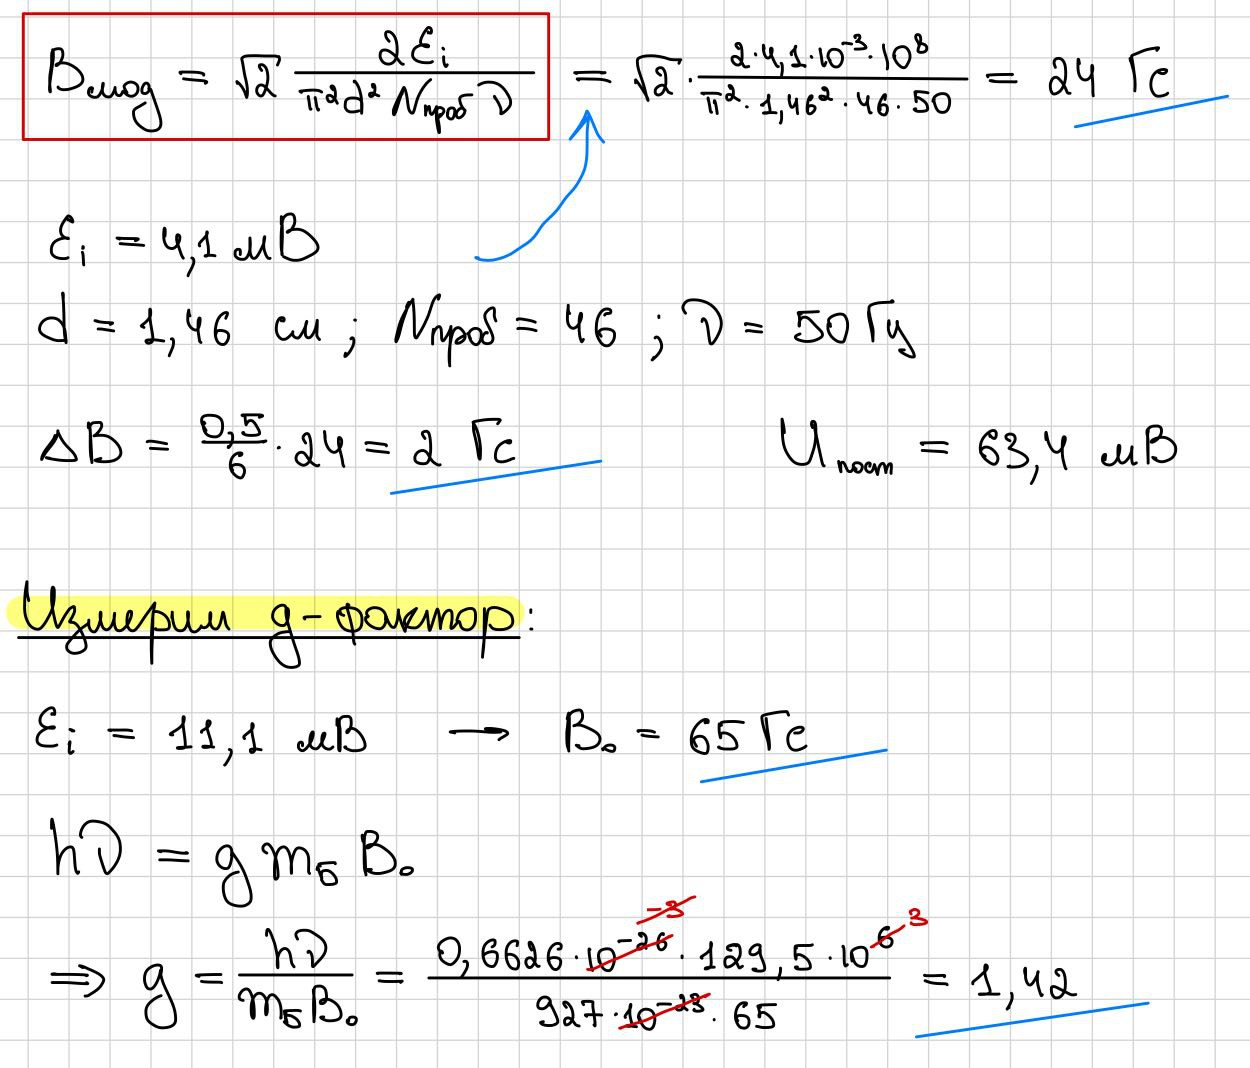
\includegraphics[width=0.7\linewidth]{res/3.png}
    \end{figure}
    
\section{Заключение}
    В заключение, хочу отметить, что мы исследовали электронный парамагнитный резонанс в молекуле ДФПГ, определили $g$-фактор электрона, измерили ширину ЭПР.
    
\end{document}
